\textbf{List the formulas you have used for the implementation of Kalman filter}\\

Implementing the extended Kalman filter for this simulation is to be done on a specific time frame of the UAV's flight - 10 minutes before the 2nd time the UAV takes off and 5 minutes after the UAV lands the 2nd time. For this time interval, begin by defining a start time (1443 seconds - 600 seconds) and an end time (1685 seconds + 300 seconds). Once this time is defined, identify the index within the time inputs to understand what index Matlab needs to begin implementing the EKF and what index it needs to stop. This is the first step in implementing the EKF.\\
To Implement an Extended Kalman Filter, begin by defining the initial state variables, the initial state covariance matrix (P), and the Measurement Covariance matrix (R):
\subsection*{State Variables}

\[
x_0 = 
\begin{bmatrix}
x_n \\
y_n \\
z_n \\
v_{x} \\
v_{y} \\
v_{z} \\
b_x \\
b_y \\
b_z
\end{bmatrix}
=
\begin{bmatrix}
x_n (@start_{time} index) \\
y_n (@start_{time} index) \\
z_n (@start_{time} index) \\
0 \\
0 \\
0 \\
0 \\
0 \\
0
\end{bmatrix}
\]\\
\textbf{Please explain the physical meanings of your state variables used in your EKF and which coordinate system they are defined in. }\\

Where $x_n$, $y_n$ and $z_n$ are the NED position coordinates, $v_x$, $v_y$, $v_z$ are the velocities of the UAV also in the NED frame, and $b_x$, $b_y$, $b_z$ are the accelerometer bias provided in the body frame.

\subsection*{State Covariance (P Matrix)}

\[
P =
\begin{bmatrix}
P_{xx} & P_{xy} & P_{xz} & P_{xv_x} & P_{xv_y} & P_{xv_z} & P_{xb_x} & P_{xb_y} & P_{xb_z} \\
P_{yx} & P_{yy} & P_{yz} & P_{yv_x} & P_{yv_y} & P_{yv_z} & P_{yb_x} & P_{yb_y} & P_{yb_z} \\
P_{zx} & P_{zy} & P_{zz} & P_{zv_x} & P_{zv_y} & P_{zv_z} & P_{zb_x} & P_{zb_y} & P_{zb_z} \\
P_{v_xx} & P_{v_xy} & P_{v_xz} & P_{v_xv_x} & P_{v_xv_y} & P_{v_xv_z} & P_{v_xb_x} & P_{v_xb_y} & P_{v_xb_z} \\
P_{v_yx} & P_{v_yy} & P_{v_yz} & P_{v_yv_x} & P_{v_yv_y} & P_{v_yv_z} & P_{v_yb_x} & P_{v_yb_y} & P_{v_yb_z} \\
P_{v_zx} & P_{v_zy} & P_{v_zz} & P_{v_zv_x} & P_{v_zv_y} & P_{v_zv_z} & P_{v_zb_x} & P_{v_zb_y} & P_{v_zb_z} \\
P_{b_xx} & P_{b_xy} & P_{b_xz} & P_{b_xv_x} & P_{b_xv_y} & P_{b_xv_z} & P_{b_xb_x} & P_{b_xb_y} & P_{b_xb_z} \\
P_{b_yx} & P_{b_yy} & P_{b_yz} & P_{b_yv_x} & P_{b_yv_y} & P_{b_yv_z} & P_{b_yb_x} & P_{b_yb_y} & P_{b_yb_z} \\
P_{b_zx} & P_{b_zy} & P_{b_zz} & P_{b_zv_x} & P_{b_zv_y} & P_{b_zv_z} & P_{b_zb_x} & P_{b_zb_y} & P_{b_zb_z}
\end{bmatrix}
= I_{9x9} (9x9 Identity Matrix)
\]\\

\textbf{Please explain what values you have chosen to initialize the state variables and the state covariance matrix P. Why these values?}\\

The state variables have been initialized with the first value of the NED positions at the provided start time, since that is what the EKF implementation required (for the UAV being 10 minutes before taking off), and therefore, using the index created with the time, we can implement that start index to capture the initial NED position of the UAV for our initial state vector. The velocities are initialized at 0 to assume that the UAV is beginning at a stationary flight, with the velocity incrementally updating through implementing EKF using accelerometer readings. If the velocity was initialized incorrectly, the beauty of EKF is that it would adjust the velocity estimates based on subsequent readings. The accelerometer bias was initialized with 0's as well since the initial bias is unknown and it is common practice to set the values to 0 and let the EKF estimate it over its iterations since the EKF will cause the bias to converge over time to the correct estimate of the bias based on the sensor readings. As more data is provided from the IMU and the GPS, the filter will help adjust the bias estimates to provide a more accurate value for the accelerometer bias, which we will show through a plot. For the state covariance, we initialize the data as a 9x9 identity matrix, with a weight of 1 provided for the diagonals of P, which is the uncertainty of each state variable ($P_{xx}, P_{yy}, P_{zz}, P_{vxvx}, P_{vyvy}, P_{vzvz}, P_{bxbx}, P_{byby}, P_{bzbz}$, where the diagonals of the P matrix = the variance of each state, and the non-diagonals = covariance. With a weight of 1, we begin by telling the system that there is a moderate degree of uncertainty for each state variable and this uncertainty is the same - a neutral, non-bias assumption of uncertainty.\\

Now, the process requires the system to be defined that we will implement EKF on to estimate the NED Position and Velocity.
\subsection*{System:}

\begin{align}
    \mathbf{x}(k+1) &= F\mathbf{x}(k) + G\mathbf{u}(k) + \mathbf{v}(k) \\
    \mathbf{y}(k) &= H\mathbf{x}(k) + \mathbf{w}(k)
\end{align}
Where the respective matrices can be computed using the process model shown below:

\subsection*{Process Model (works for navigation within small earth surface area)}

\[
\begin{bmatrix}
x \\
y \\
z \\
v_x \\
v_y \\
v_z \\
b_x \\
b_y \\
b_z
\end{bmatrix}_{k+1}
=
\underbrace{
\begin{bmatrix}
1 & 0 & 0 & dt & 0 & 0 & -dt^2/2 & 0 & 0 \\
0 & 1 & 0 & 0 & dt & 0 & 0 & -dt^2/2 & 0 \\
0 & 0 & 1 & 0 & 0 & dt & 0 & 0 & -dt^2/2 \\
0 & 0 & 0 & 1 & 0 & 0 & -dt & 0 & 0 \\
0 & 0 & 0 & 0 & 1 & 0 & 0 & -dt & 0 \\
0 & 0 & 0 & 0 & 0 & 1 & 0 & 0 & -dt \\
0 & 0 & 0 & 0 & 0 & 0 & 1 & 0 & 0 \\
0 & 0 & 0 & 0 & 0 & 0 & 0 & 1 & 0 \\
0 & 0 & 0 & 0 & 0 & 0 & 0 & 0 & 1
\end{bmatrix}
}_{F}
\begin{bmatrix}
x \\
y \\
z \\
v_x \\
v_y \\
v_z \\
b_x \\
b_y \\
b_z
\end{bmatrix}_k
+
\underbrace{
\begin{bmatrix}
\frac{dt^2}{2} & 0 & 0 \\
0 & \frac{dt^2}{2} & 0 \\
0 & 0 & \frac{dt^2}{2} \\
dt & 0 & 0 \\
0 & dt & 0 \\
0 & 0 & dt \\
0 & 0 & 0 \\
0 & 0 & 0 \\
0 & 0 & 0 
\end{bmatrix}
}_{G}
\begin{bmatrix}
R_{g/b} \\
0 \\
g
\end{bmatrix}
\begin{bmatrix}
a_x \\
a_y \\
a_z \\
1
\end{bmatrix}_k
\]

Where $(R_{g/b})$ is a rotation matrix to convert the values from the body frame to the ground frame.

\[
R_{g/b} = 
\begin{pmatrix}
\dot{X}_n \\
\dot{Y}_n \\
\dot{Z}_n
\end{pmatrix}
=
\begin{bmatrix}
c_\psi c_\theta & c_\psi s_\theta s_\phi - s_\psi c_\phi & c_\psi s_\theta c_\phi + s_\psi s_\phi \\
s_\psi c_\theta & s_\psi s_\theta s_\phi + c_\psi c_\phi & s_\psi s_\theta c_\phi - c_\psi s_\phi \\
-s_\theta       & c_\theta s_\phi                         & c_\theta c_\phi
\end{bmatrix}
\begin{pmatrix}
u \\
v \\
w
\end{pmatrix}
\]

\subsection*{Process Noise Covariance}

\[
Q = G
\begin{bmatrix}
q_x & 0 & 0 & 0 \\
0 & q_y & 0 & 0 \\
0 & 0 & q_z & 0 \\
0 & 0 & 0 & 0
\end{bmatrix}
G' = 
G
\begin{bmatrix}
0.7 & 0 & 0 & 0 \\
0 & 0.4 & 0 & 0 \\
0 & 0 & 1.5 & 0 \\
0 & 0 & 0 & 0
\end{bmatrix}
G'
\]

\subsection*{Measurement Noise Covariance (R Matrix)}

\[
R =
\begin{bmatrix}
R_{xx} & 0      & 0      \\
0      & R_{yy} & 0      \\
0      & 0      & R_{zz}
\end{bmatrix}
= 
\begin{bmatrix}
eph & 0      & 0      \\
0      & eph & 0      \\
0      & 0      & epv
\end{bmatrix} * 1e-3
\]

\subsubsection*{1. Predict}

\begin{align}
    \hat{\mathbf{x}}(k+1 | k) &= F \hat{\mathbf{x}}(k | k) + G\mathbf{u}(k) \\
    P(k+1 | k) &= F P(k | k) F^T + Q
\end{align}

\subsubsection*{2. Correction}

\begin{align}
    S &= H P(k+1 | k) H^T + R \\
    W &= P(k+1 | k) H^T S^{-1} \\
    \Delta \mathbf{x} &= W \left( \mathbf{y}(k+1) - H \hat{\mathbf{x}}(k+1 | k) \right)
\end{align}

\subsubsection*{3. Update}

\begin{align}
    \hat{\mathbf{x}}(k+1 | k+1) &= \hat{\mathbf{x}}(k+1 | k) + W \mathbf{v} \\
    P(k+1 | k+1) &= P(k+1 | k) - W S W^T
\end{align}
Where H is the measurement matrix relating the state vector to the measurements, mapping the state space to the measurement space. The matrix H in our system is given by:
\begin{align*}
    H = \begin{bmatrix}
    1 & 0 & 0 & 0 & 0 & 0 & 0 & 0 & 0 \\
    0 & 1 & 0 & 0 & 0 & 0 & 0 & 0 & 0 \\
    0 & 0 & 1 & 0 & 0 & 0 & 0 & 0 & 0
    \end{bmatrix}
\end{align*}

\textbf{Explain the choice of Q and R matrices for EKF implementation.}\\

Initially, I defined the Q matrix with 1's in the $q_x, q_y, q_z$ diagonals, and the R matrix to be the horizontal and vertical variance from the GPS since GPS measurements are the most accurate. Using these initial values of Q and R, I defined the process and implemented the EKF using just GPS readings to see if my Q and R matrix of the model was accurate. The first attempt showed that there was a lot of drift in my EKF estimated position, as well as velocity. Therefore I knew that I had to tune my Q and R matrix to allow my EKF estimation to better match my NED positions from GPS raw measurements. The tuning process for both Q and R were a little different since each matrix affected the system differently. I started by focusing on Q. The Q matrix - process noise covariance supports the system by defining the uncertainty in the IMU measurements from the accelerometer. Theoretically, if the weight on Q was too large, EKF would result in trusting the IMU readings more than it should, resulting in a greater drift, and if the value was too small, then the GPS readings would be trusted more, producing greater noise in the system. Therefore, knowing that GPS was the most accurate reading I had, I reduced my Q from 1's to decimals (i.e., 0.7, 0.4, 1.5), which provided a more accurate estimation from EKF to the GPS to NED measurements. Once I was able to tune Q, it was time to focus on R - the measurement noise covariance. R is used to define the uncertainty present in our GPS data, which means that the more noisy the GPS data is, the better R can help in reflecting the actual noise characteristics of GPS. Theoretically, increasing R would result in EKF not trusting GPS measurements as much, and reducing R would cause the system to trust the noisy GPS data more. Therefore, from trial and error of different values, I was able to capture an R matrix that better estimated my NED position with the GPS horizontal and vertical covariance values being reduced by 1e-3.\\

Once I was able to define a Q and R matrix that was able to estimate NED position and velocity accurately, I could address the issue of the difference in GPS and IMU update rates.\\

\textbf{GPS update rate is slower than IMU update rate, explain how you implemented code to address this practical issue.}\\

Since the GPS update rate is slower than the IMU update rate, I decided to not take all GPS inputs to update the prediction step of the NED position estimate and to instead use a time gap (i.e., take fewer GPS inputs to allow for correction and update step to match IMU better). This time gap was selected to be every 2nd GPS input for 1 IMU update (e.g., 1st update step using IMU, 2nd update step comes from correction step with GPS update, and then an update step using GPS). The value of using every 2nd GPS input vs. 5th or 10th was done using an iterative process, where the process began without skipping some GPS values (i.e, mod (i,1) == 0) to see the estimation of NED positions implementing EKF. From skipping no values, we iterated by increasing the # of GPS inputs being skipped up until 10. As the # of inputs being skipped increased over 4, the estimation started to produce a larger drift for the NED positions. This resulted in the final implementation to capture every 2nd GPS input into correction and update step of the EKF implementation to produce the figure shown below.\\
This implementation of not updating every prediction value using GPS input allowed to estimate the NED positions with more accuracy as shown in the plot below. It is visible that EKF implementation (shown through the Black line) is mimicking the NED positions from GPS (shown through the dotted red line). 

\begin{figure}[H]
  \centering
 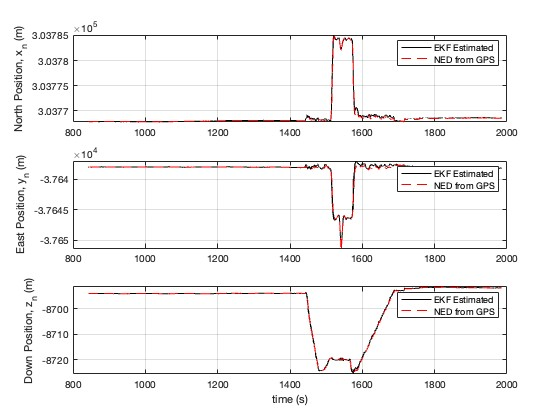
\includegraphics[width=0.8\linewidth, height=0.7\linewidth]{EKF/EKF_Pos.jpg}  
\caption{NED Positions Estimated from EKF Implementation}
\label{fig:EKFPos}
\end{figure}
\\
Since the state estimate also provided us with velocity and acceleration bias, to compare the velocity from the GPS-derived NED positions, we differentiated the NED positions from raw GPS measurement. First, define the time derivative $dt_v$ which is the derivative of the time-interval for the UAV's 2nd flight, which was 10 minutes before taking off and 5 minutes after landing. To calculate the velocity, we differentiate the NED positions from the start-to-end index defined for our EKF implementation and we divide it by $dt_v$.
\begin{align*}
    \Delta t_v &= \text{diff}( \text{time\_int} ) \\
    v_n &= \frac{\text{diff}(x_n( \text{start\_i} : \text{end\_i}))}{\Delta t_v} \\
    v_e &= \frac{\text{diff}(y_n( \text{start\_i} : \text{end\_i}))}{\Delta t_v} \\
    v_d &= \frac{\text{diff}(z_n( \text{start\_i} : \text{end\_i}))}{\Delta t_v} \\
\end{align*}\\
Since the Velocity of the UAV from NED was captured through differentiating the NED positions, the EKF estimation of velocity uses both IMU data and GPS data to estimate velocity, while accounting for sensor noise and drift. It filters the noise through using the process model and Kalman gain, allowing an estimation of a smoother and less noisy velocity estimate in comparison to the differentiated NED position - velocity. Since the EKF incorporates bias correction, the EKF is able to correct the velocity estimate based on accelerometer bias over time allowing it to reduce the impact of the sensor's drift on the estimated velocity, providing a more accurate velocity reading. NED-differentiated velocity is more accurate when the GPS data is more frequent and with minimal noise, but when the motion is fast or involves frequent changes in velocity, the EKF is more accurate due to the high IMU update rate. In our case, the EKF estimated velocity is more accurate and can be seen from the graph below.

\begin{figure}[H]
  \centering
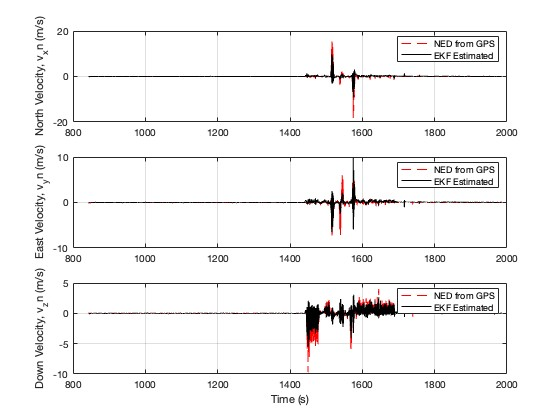
\includegraphics[width=0.8\linewidth, height=0.7\linewidth]{EKF/EKF_Vel.jpg}  
\caption{NED Velocity Estimated from EKF Implementation}
\label{fig:EKFVel}
\end{figure}

You can find below the code used to implement EKF and produce the necessary graphs in section 5, Implementing Extended Kalman Filter for NED Position and Velocity.
\label{EKF Estimated NED Matlab Code}
\begin{lstlisting}
% Implementing EKF for time 2nd UAV take-off and landing where t_min is 10 minutes before UAV taking off and t_max is 5 minutes after landing. From Motor Signal, we can see that UAV took off at 1440 seconds, and landed at 1695 seconds

% Define time interval as provided in the problem statement and define time index to synchronize data between GPS and IMU to align readings based on timestamp
start_t = 1443 - 600; % 10 min before taking-off a second time
start_i = find(t>= start_t,1); % Start time index
end_t = 1685 + 300; % 5 min after landing a second time
end_i = find(t>= end_t,1); % End time index
time_int = t(start_i:end_i); % Define time values from time dataset

% State Variables of interest [NED Position, NED Velocity, Accelerometer Bias]
% x = [x_n, y_n, z_n, v_x, v_y, v_z, b_x, b_y, b_z]
% Define initial state, covariance, and measurement noise covariance
x0 = [x_n(start_i); y_n(start_i); z_n(start_i); 0; 0; 0; 0; 0; 0]; % State
P0 = eye(9); % Covariance
R = diag([eph,eph,epv]) * 1e-3; % Measurement noise covariance, GPS is most reliable
x_hat = zeros(9, length(time_int)); % Create arrays for NED estimate coordinates

% Implementing Extended Kalman Filter - Create System Matrices
for i = start_i:end_i
    dt = (time_int(end) - time_int(1))/(length(time_int)); % Assuming uniform sampling

    % Create Rotation Matrix to move from NED to Ground Frame
    R_NEDtoGround = [cos(psi(i)) * cos(tht(i)) , (cos(psi(i)) * sin(tht(i)) * sin(phi(i))) - (sin(psi(i)) * cos(phi(i))) , (cos(psi(i)) * sin(tht(i)) * cos(phi(i))) + (sin(psi(i)) * sin(phi(i)));
    sin(psi(i)) * cos(tht(i)) , (sin(psi(i)) * sin(tht(i)) * sin(phi(i))) + (cos(psi(i)) * cos(phi(i))) , (sin(psi(i)) * sin(tht(i)) * cos(phi(i))) - (cos(psi(i)) * sin(phi(i)));
    -sin(tht(i)),  cos(tht(i)) * sin(phi(i)),  cos(tht(i)) * cos(phi(i))];
    
    % Create the State Transition Matrix
    F_1 = [eye(3), diag([dt, dt, dt]) , diag([(-dt^2)/2, (-dt^2)/2, (-dt^2)/2]); 
           zeros(3,3) , eye(3), diag([-dt, -dt, -dt])];
    F_2 = [eye(6), zeros(6,3);
           zeros(3,6) , R_NEDtoGround];
    F = [F_1 * F_2         ;  % Upper region of F
         zeros(3,6), eye(3)]; % Lower region of F

    % Define gravity for G matrix
    g = 9.81; % m/s^2

    % Create the Control Input Matrix
    G_1 = [diag([(dt^2)/2, (dt^2)/2 , (dt^2)/2]);
           diag([  dt    ,    dt    ,   dt    ]);
                          zeros(3,3)           ];
    G_2 = [R_NEDtoGround, [0 ; 0 ; g]];
    G = G_1 * G_2;

    % Create process noise covariance matrix
    Q = G * diag([0.7 , 0.4 , 1.5 , 0]) * G'; %qx, qy, qz

    % Prediction Step - using the previous time step to produce an estimation of the state at the current time step
    x_pred = (F * x0) + (G * [acx(i) ; acy(i) ; acz(i) ; 1]);
    P_pred = (F * P0 * F') + Q;

    % Defining the Measurement Model of GPS
    y = [x_n(i+1) ; y_n(i+1) ; z_n(i+1)];

    % To account for the difference in GPS update rate and IMU update rate, need to input a condition such that the GPS update rate is lower to provide long-term position accuracy
    if mod(i, 2) == 0
        % Correction Step with GPS update (every 3rd iteration)
        H = [eye(3), zeros(3, 6)]; % Output Matrix
        S = (H * P_pred * H') + R; % Residual covariance
        W = P_pred * H' * inv(S);  % Optimal Kalman Gain

        % Update step using GPS
        x0 = x_pred + (W * (y - (H * x_pred)));
        P0 = (eye(9) - (W * H)) * P_pred;
        
    else
        % Update step without GPS (IMU update)
        x0 = x_pred;
        P0 = P_pred;
    end

    % Store estimates
    x_hat(:,i) = x0;
end   

% Extract estimated velocities
x_hat = x_hat(:,start_i:end_i);
EKF_pos_N = x_hat(1, :); EKF_pos_E = x_hat(2, :); EKF_pos_D = x_hat(3, :);
EKF_vel_N = x_hat(4, :); EKF_vel_E = x_hat(5, :); EKF_vel_D = x_hat(6, :);
EKF_bx = x_hat(7, :); EKF_by = x_hat(8, :); EKF_bz = x_hat(9, :);

% Calculate NED Velocity and Acceleration from GPS Measurement
dt_v = diff(time_int); dt_a = diff(dt_v);
v_n = diff(x_n(start_i:end_i))./dt_v; a_n = diff(v_n)./dt_a;
v_e = diff(y_n(start_i:end_i))./dt_v; a_e = diff(v_e)./dt_a;
v_d = diff(z_n(start_i:end_i))./dt_v; a_d = diff(v_d)./dt_a;

%% Plot of estimated NED positions based on EKF vs. time
figure; set(gcf,'numbertitle','off','name','EKF Estimated NED Positions');  
subplot(3,1,1); plot(time_int, EKF_pos_N, 'k', time_int, x_n(start_i:end_i), 'r--' ); legend('EKF Estimated', 'NED from GPS');ylabel('North Position, x_n (m)'); grid on;
subplot(3,1,2); plot(time_int, EKF_pos_E, 'k', time_int, y_n(start_i:end_i), 'r--' ); legend('EKF Estimated', 'NED from GPS');ylabel('East Position, y_n (m)'); grid on;
subplot(3,1,3); plot(time_int, EKF_pos_D, 'k', time_int, z_n(start_i:end_i), 'r--' ); legend('EKF Estimated', 'NED from GPS');ylabel('Down Position, z_n (m)'); grid on; xlabel('time (s)');

%% Estimated NED velocities based on EKF Implementation againt time
figure; set(gcf,'numbertitle','off','name','EKF Estimated NED Velocity');  
subplot(3,1,1); plot(time_int(2:end), v_n, 'r--', time_int, EKF_vel_N, 'k' ); legend('EKF Estimated', 'NED from GPS');ylabel('North Velocity, v_xn (m/s)'); grid on;
subplot(3,1,2); plot(time_int(2:end), v_e, 'r--', time_int, EKF_vel_E, 'k' ); legend('EKF Estimated', 'NED from GPS');ylabel('East Velocity, v_yn (m/s)'); grid on;
subplot(3,1,3); plot(time_int(2:end), v_d, 'r--', time_int, EKF_vel_D, 'k'); legend('EKF Estimated', 'NED from GPS');ylabel('Down Velocity, v_zn (m/s)'); grid on; xlabel('Time (s)');

%% Plot of Local NED Acceleration being converted from GPS vs. time
figure; set(gcf,'numbertitle','off','name','NED Acceleration from GPS');  
subplot(3,1,1); plot(time_int(3:end), a_n);ylabel('North Acceleration (a_n, m/s^2)'); grid on;
subplot(3,1,2); plot(time_int(3:end), a_e);ylabel('East Acceleration (a_e, m/s^2)'); grid on;
subplot(3,1,3); plot(time_int(3:end), a_d);ylabel('Down Acceleration (a_d, m/s^2)'); grid on; xlabel('time (s)');

%% Plot of Accelerometer bias from EKF Implementation against time
figure; set(gcf,'numbertitle','off','name','EKF Estimated Accelerometer Bias');  
subplot(3,1,1); plot(time_int, EKF_bx);ylabel('EKF Estimated b_x (m/s^2)'); grid on;
subplot(3,1,2); plot(time_int, EKF_by);ylabel('EKF Estimated b_y (m/s^2)'); grid on;
subplot(3,1,3); plot(time_int, EKF_bz);ylabel('EKF Estimated b_z (m/s^2)'); grid on; xlabel('time (s)');
\end{lstlisting}
\captionof{figure}{MATLAB Code for Implementing EKF to Estimate NED Positions and Velocity}
\label{fig:EKF2NED}

